\chapter{Introduction}

\section{INGInious}

INGInious is a web platform developped by the UCL.  It is a tool for automatic correction of programs written by students.  It currently relies on Docker containers to provide a good isolation between the machine hosting the site and the execution of the student's codes.  So that a problem in a program submitted by a student couldn't have any impact on the platform.  Docker also allow to manage the resources granted to each code execution.  For now INGInious can meet the demand and provide honest performances and responsiveness.  But looking at the growing usage of the platform, we might soon come to a point where we reach the limits of the current implementation.

\subsection{Architecture}
INGInious counts four main components:
\begin{enumerate}
  \item The front-end: the website with which each student interacts when submitting a task.
  \item The back-end: a queue of all the tasks that need to be graded.
  \item The docker agent: responsible for the container assignment to the pending tasks when resources are available.
  \item The docker containers: one for the student code and one for the teacher tests evaluating the student's code behaviour.
\end{enumerate}
The journey of a task submitted on INGInious is represented on Figure \ref{fig:architecture}.
\begin{figure}[!h]
  \begin{center}
    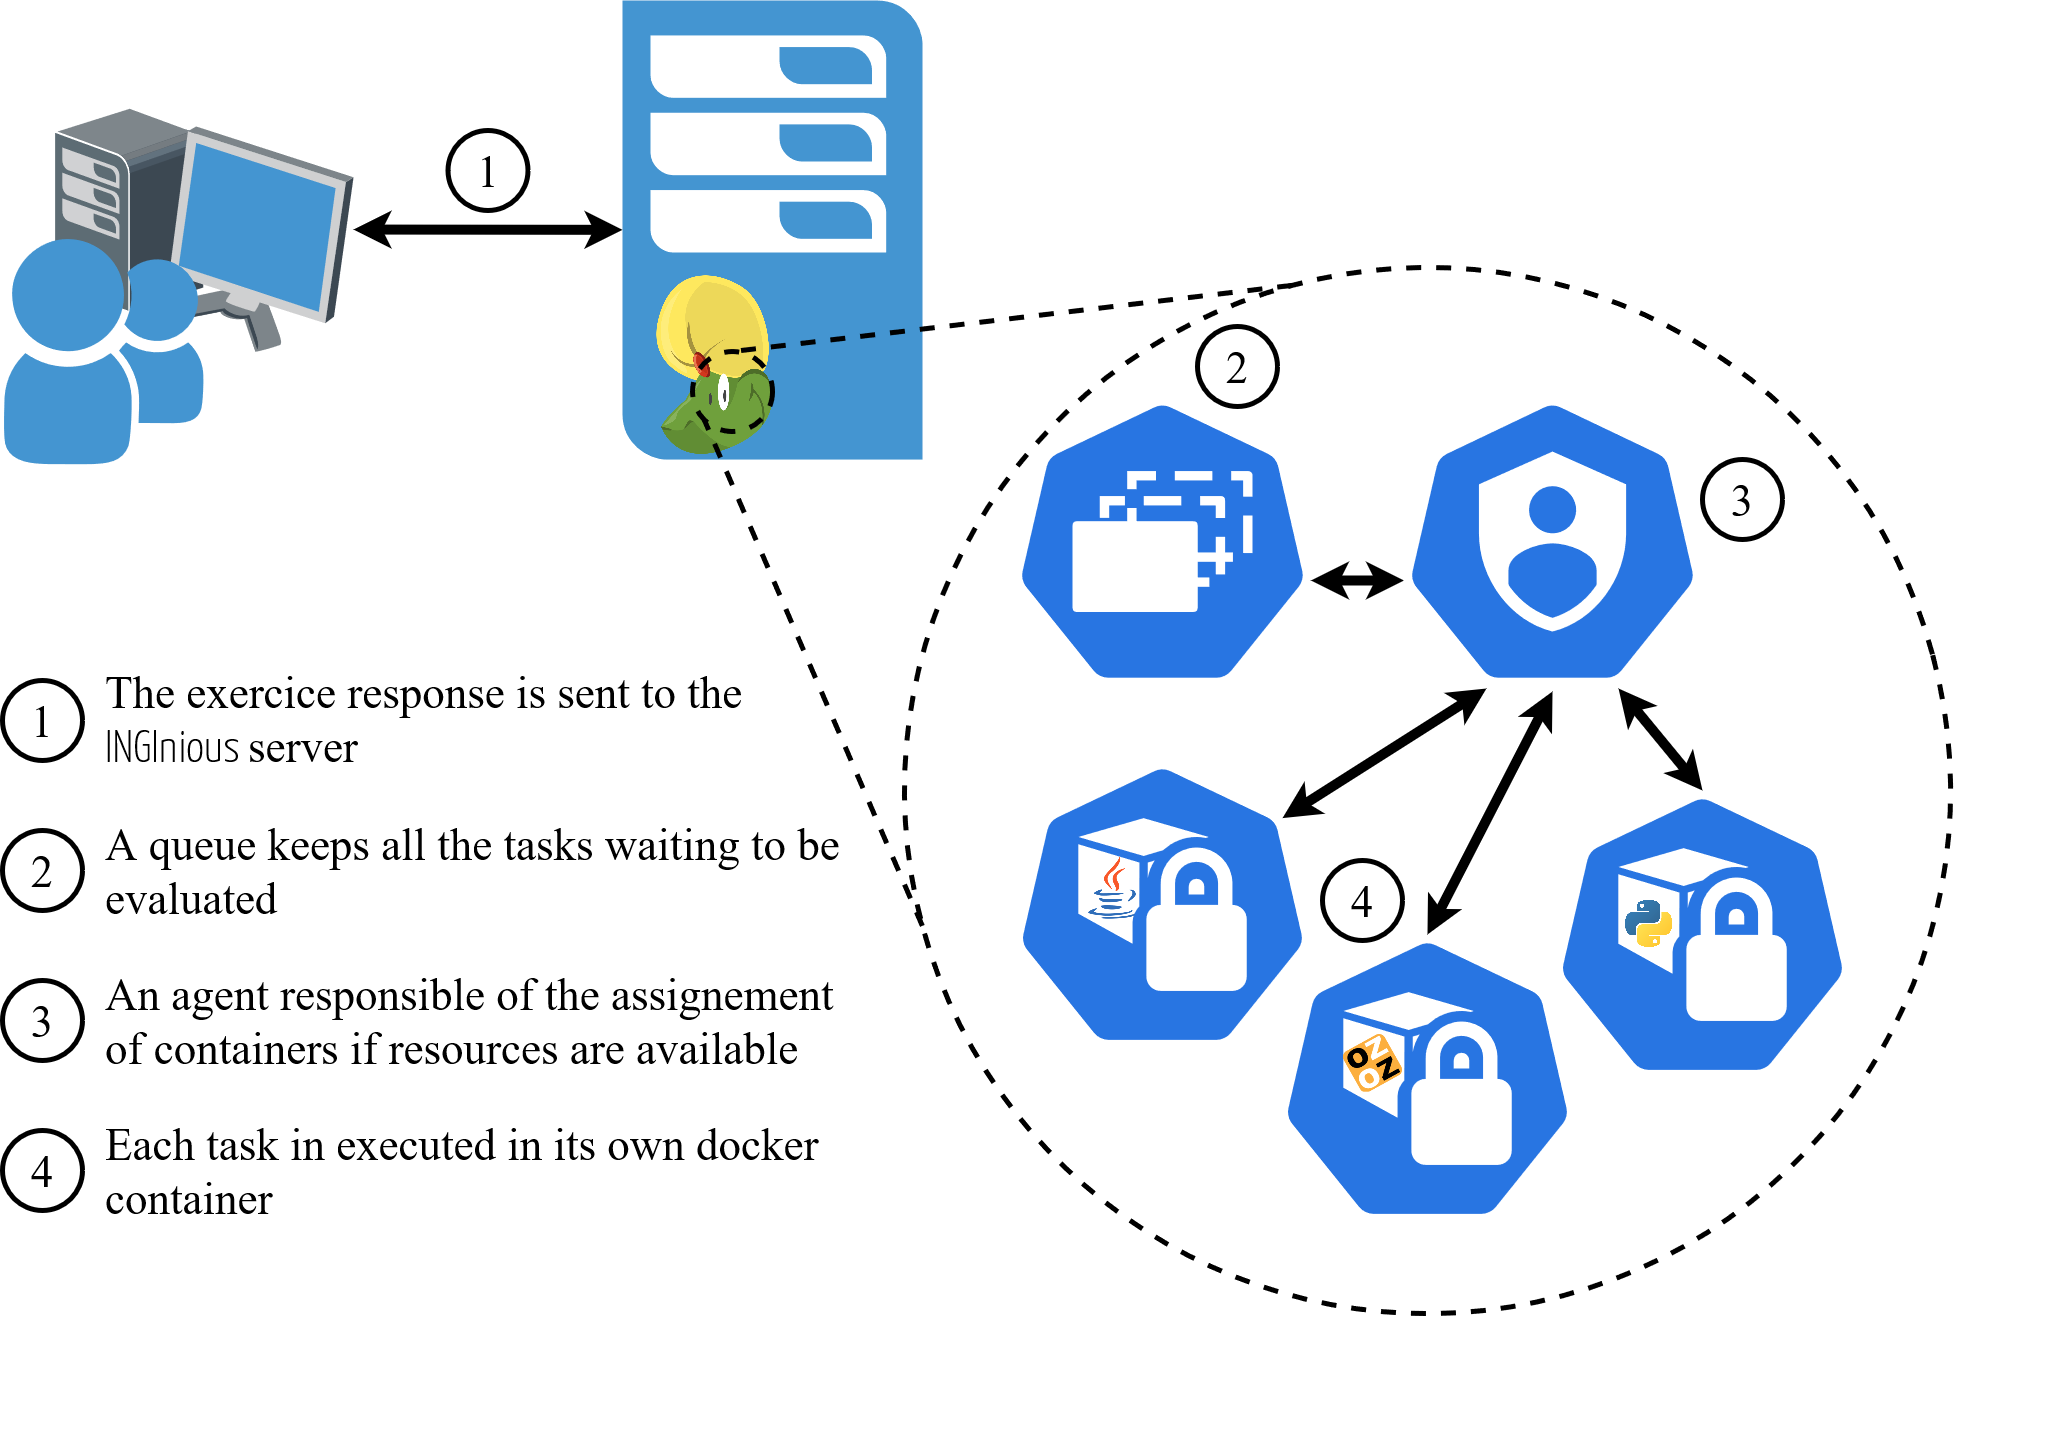
\includegraphics[width=\linewidth]{images/Architecture.png}
    \caption{INGInious global architecture}
    \label{fig:architecture}
  \end{center}
\end{figure}

\subsection{Key features}

\subsection{Bottlenecks}

\section{Scaling}
Currently, the resources provided to INGInious vary depending on the load that the platform is expected to be facing.  Typically, when the grading of an exam is done by INGInious, the platform is scaled up, and during the holidays it is scaled down.  
In general, the scaling can be done in two directions, horizontally, or vertically.

\subsection{Vertical scaling}

\subsection{Horizontal scaling}

\section{Intentions}
